The benchmark  

The retrieval performance of submitted results has been evaluated using 7 commonly used retrieval performance metrics. The publicly available benchmark~\cite{SHREC18-SceneSBR-Track}, comparative evaluation results and corresponding evaluation code will enrich and advance the research of 2D scene sketch-based 3D scene retrieval and its applications.



\paragraph{Preliminary Work.} 
To advance this promising research, we organized a challenge on 2D Scene Image-Based 3D Scene Retrieval~\cite{DBLP:conf/3dor/AbdulJLL18, SHREC18-SceneIBR-Track} in the 2018 Shape Retrieval Contest (SHREC) which is in conjunction with the Eurographics 2018 Workshop on 3D Object Retrieval (3DOR'18) and built the first 2D scene image-based 3D scene retrieval benchmark \textbf{SceneIBR} by collecting 2D images from ImageNet and 3D scenes from 3D Warehouse~\cite{3DWarehouse}. The benchmark contains uniformly classified 10,000 2D scene images and 1,000 3D scene models of ten (10) categories. In this track, seven (7) groups from five countries (China, Chile, USA, UK, and Vietnam) registered for the track, while due to many challenges involved, only three (3) groups successfully submitted ten (10) runs of five methods. To have a comprehensive comparison, seven (7) commonly-used retrieval performance metrics have been used to evaluate their retrieval performance. The publicly available~\cite{SHREC18-SceneIBR-Track} benchmark, comparative evaluation results and corresponding evaluation code, will further enrich and boost the research of 2D scene image-based 3D scene retrieval and its applications.



%%%%%%%%%%%%%%%%%%%Introduction%%%%%%%%%%%%%%%%
To advance this promising research, we organize this SHREC track and build the first 2D scene image-based 3D scene retrieval benchmark by collecting 2D images from ImageNet and 3D scenes from Google 3D Warehouse. The benchmark contains uniformly classified 10,000 2D scene images and 1,000 3D scene models of ten (10) categories. In this track, seven (7) groups from five countries (China, Chile, USA, UK, and Vietnam) have registered for the track, while due to many challenges involved, only three (3) groups have successfully submitted ten (10) runs of five methods. To have a comprehensive comparison, seven (7) commonly-used retrieval performance metrics have been used to evaluate their retrieval performance. We also suggest several future research directions for this research topic. We wish this publicly available~\cite{SHREC18-SceneIBR-Track} benchmark, comparative evaluation results and corresponding evaluation code, will further enrich and boost the research of 2D scene image-based 3D scene retrieval and its applications.



Therefore, this research topic deserves our further exploration.



In fact, due to the even bigger representation gap between rough 2D scene sketch representation and accurate 3D scene model coordinates, 2D scene sketch-based 3D model retrieval (SceneSBR) is one of the most challenging research topics in the field of 3D scene retrieval. 

2D Scene-based 3D scene retrieval is a brand new research topic in the field of 3D
object retrieval. 

2D scene-based 3D model retrieval has the intuitiveness advantage over other types of retrieval schemes. Currently, there is a lot
of research in object-based 3D model retrieval, which usually targets the problem of retrieving a list of candidate 3D models
using a single 2D image as input. 



Unlike traditional object-based 3D model retrieval which ideally assumes that a query 2D image contains only a
single object, this is a new 3D model retrieval topic within the context of a 2D scene which contains several objects that
may overlap with each other and thus be occluded and also have relative location configurations. It is challenging due to the
semantic gap existing between the iconic 2D representation of 2D scene image and more accurate 3D representation of 3D models.



%%%%%%%%%%%%%%%%%%%%%%%%%%%%%%%%%
%%%%%%%   Contribution
%%%%%%%%%%%%%%%%%%%%%%%%%%%%%%%%%
%\paragraph{Problem $\&$ Significance.}
\paragraph{Research Goal $\&$ Approach.}
Therefore, now we can find that there is either a big \textbf{semantic gap} between 2D scene sketches and 3D scene models for 2D scene sketch-based 3D scene shape retrieval, or a scarce of substantial research in 2D scene image-based 3D scene shape retrieval due to its \textbf{challenges and difficulties}. 

To our best knowledge, this project is the \textbf{first} attempt to explore 2D scene sketches/images and 3D scenes matching at semantic level with a tree structure and to develop a comprehensive framework to perform the 3D scene retrieval. The implication of this work could not only accelerate the research on sketch/image-based 3D scene retrieval, but also shed inspiring light on 2D/3D scene understanding related research work. Our main goals to be achieved in this project are listed as follows:

\begin{itemize}

\item A huge comprehensive \textbf{scene semantic tree} will be created based on WordNet. We plan to collect a large amount of 2D/3D scenes to build the currently largest and only available scene semantic tree which accommodates  more than 10 million 2D/3D scene files (images, sketches, and models) around 500 categories. In detail, it has about half million 3D scene models (1K models per class, in average), 5 million 2D scene images (10K images per class, in average), and 5 million 2D scene sketches (10K sketches per class, in average). It will be a pioneer work to lead this semantics-driven 3D scene retrieval research. 

\item A novel \textbf{semantic tree-based 3D scene retrieval framework} is proposed. This approach will capture semantic information of 2D sketches/images or 3D scene models effectively, measure similarities between semantics of 2D sketches/images and 3D scenes accurately, and therefore greatly enhance the retrieval performance. The proposed sketch/image-based 3D scene retrieval framework will benefit many potential applications including virtual reality, gaming, 3D movie, and mobile apps etc. 


\item Extensive \textbf{application} research of our semantics-driven 3D shape retrieval framework is proposed, especially in 1) semantics-driven 2D scene sketch/image based 3D scene retrieval, and 2) semantics-driven 2D scene sketch-based 3D scene reconstruction. 


\item The scene semantic tree to be built in this project will provide a very useful \textbf{scene semantics infrastructure} for many related applications. Our work will explicitly guide the research on sketch/image-based 3D scene retrieval and also provide a direction for related 2D and/or 3D scene understanding applications, including object detection, as well as scene classification, recognition, and retrieval. 

%First, we will further extend the 3D semantic tree to accommodate other types of shape data, such as 3D scene models, and 2D scene sketches/images. Then, we adapt the proposed semantic tree-based 3D scene retrieval framework for related applications research in the following areas: 1) semantics-driven 2D image-based 3D scene retrieval, 2) semantics-driven 2D scene sketch-based 3D scene retrieval, and 3) semantics-driven 2D scene sketch-based 3D scene reconstruction.

%The proposed novel semantic tree-based 3D scene retrieval framework will explicitly guide the research on sketch-based 3D scene retrieval and also provide a direction for sketch-based related applications and benefit many potential applications including virtual reality, gaming, 3D movie, and mobile apps. 


%\item \textcolor{red}{Educations? SHRECs?}


%\item

\end{itemize}


%%%%%%%%%%%%%%%%%%%%%%%%%%%%%%%%%%%%%%%%%%%
\subsection{2D/3D scene benchmarks} %: techniques and benchmarks

\subsubsection{Xiao et. al's SUN and SUN3D databases (2010, 2016)}
Xiao et. al~\cite{DBLP:conf/cvpr/XiaoHEOT10} built the Scene UNerstanding (SUN) image database for the purpose of fostering improvements in  large scale scene recognition. SUN was initially comprised of 899 scene categories and 130,519 images. Later, SUN was extended to include 908 distinct classes \cite{DBLP:journals/ijcv/XiaoEHTO16}. Xiao et. al~\cite{DBLP:conf/iccv/XiaoOT13} further created SUN3D, a RGB-D video database with camera pose and
object labels, to capture full extend of 3D places. They used the videos for partial 3D reconstruction and propagated labels from one frame to another, then used the labels to refine the partial reconstruction. %This is achieved by using object-to-object correspondences in the bundle adjustment step of reconstruction. SUN3D achieved its goal to improve the accuracy of structure from motion while reducing the amount of hand labeling needed between video frames.  

\subsubsection{Hua et. al's SceneNN dataset (2016)}
Hua et. al~\cite{DBLP:conf/3dim/HuaPNTYY16} released SceneNN, a richly annotated RGB-D indoor scene dataset which contains 100 scenes annotated at the vertex, mesh and pixel level. This level of detail in annotation is in hope to promote research in various computer vision and scene understanding applications.


\subsubsection{Xiang et. al's ObjectNet3D database  (2016)}
Xiang et. al~\cite{DBLP:conf/eccv/XiangKCJCSMGS16} curated ObjectNet3D, a large 3D scene dataset across 100 categories. The dataset is comprised of 90,127 scene images, 201,888 objects within the scene images and 44,147 3D objects. ObjectNet3D aligns 2D images with 3D shapes, provides 3D pose annotations and approximate 3D shape annotations. ObjectNet3D's goal is to provide annotations at a large scale comparable to that of recent 2D datasets.

\subsubsection{Handa et. al's SceneNet network and dataset (2016)}
Handa et. al~\cite{DBLP:conf/icra/HandaPSC16} designed SceneNet, a framework that automatically generates much needed labeled training data  for 3D scene understanding, such as synthetic 3D scenes as well as RGB-D videos with semantic annotations. SceneNet utilizes 57 hand created scenes across 5 indoor scene categories and leverages existing indoor scene annotations to find correlation and semantics between objects. Once relationships of objects are extracted, SceneNet samples CAD repositories and constructs a new synthetic scene with annotations. Finally, they generated around 10k synthetic views for the five types of 3D scenes for different scene understanding experiments. 

\subsubsection{Song et. al's SUNCG database (2017)}
Song et. al~\cite{DBLP:conf/cvpr/SongYZCSF17} constructed SUNCG,  a database of synthetic 3D scenes with manually labeled voxel occupancy and semantic labels. SUNCG has 45,622 different scenes and 2,644 objects across 84 categories. They also developed the Semantic Scene Completion Network (SSCNet), an end-to-end 3D convolutional neural network, which uses a single depth image as input and produces semantic labels as well as a voxel occupancy grid. They trained SSCNet with SUNCG, and achieved state-of-the-art performance in both scene completion and semantic labeling. 


\subsubsection{Zhou et. al's Places database (2018)}
Zhou et. al~\cite{DBLP:journals/pami/ZhouLKO018} compiled Places, a database of 10,624,928 scene images across 434 scene categories. While Places is not annotated at the object level, it provides the most diverse scene composition as well as insights into solutions to scene understanding problems.


\subsubsection{Zou et. al's SketchyScene dataset (2018)}
Zou et. al~\cite{zou_eccv18} curated SketchyScene, a dataset with 29,000 scene-sketches, over 7,000 pairs of scene templates and photos, and  over 11,000 object sketches. Each scene is comprised of object-based semantic ground truths and instance mask. They also provided insights into the use of SketchyScene to explore potential methods trained to perform semantic segmentation as well as image retrieval, captioning and sketch coloring.




\begin{figure}[t]
\centering
\subfigure[Example 2D scene sketches]
{
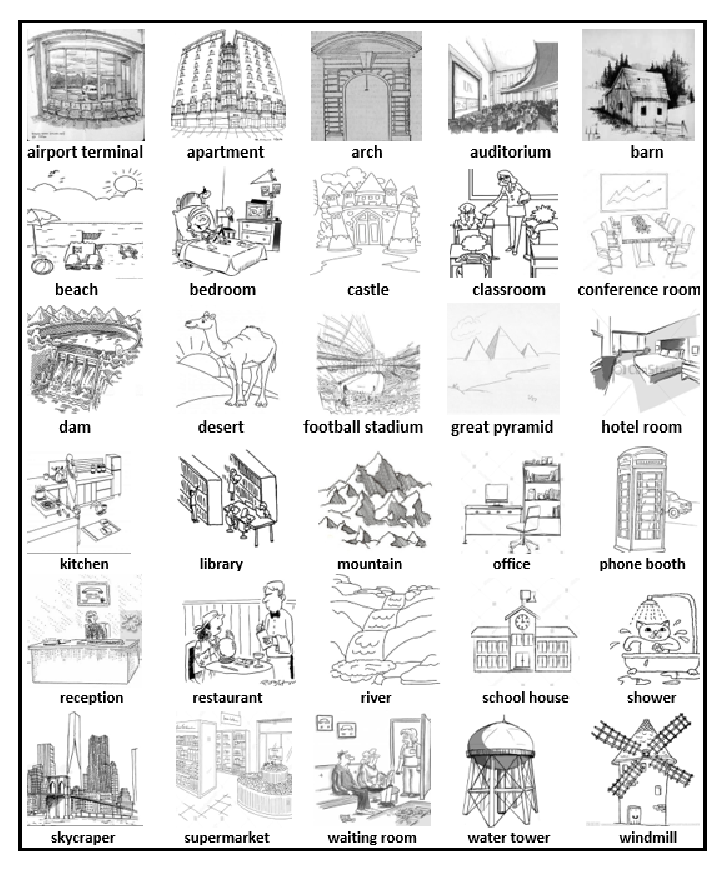
\includegraphics[width=0.7\linewidth]{SampleSketches}
}
\subfigure[Example 2D scene images]
{
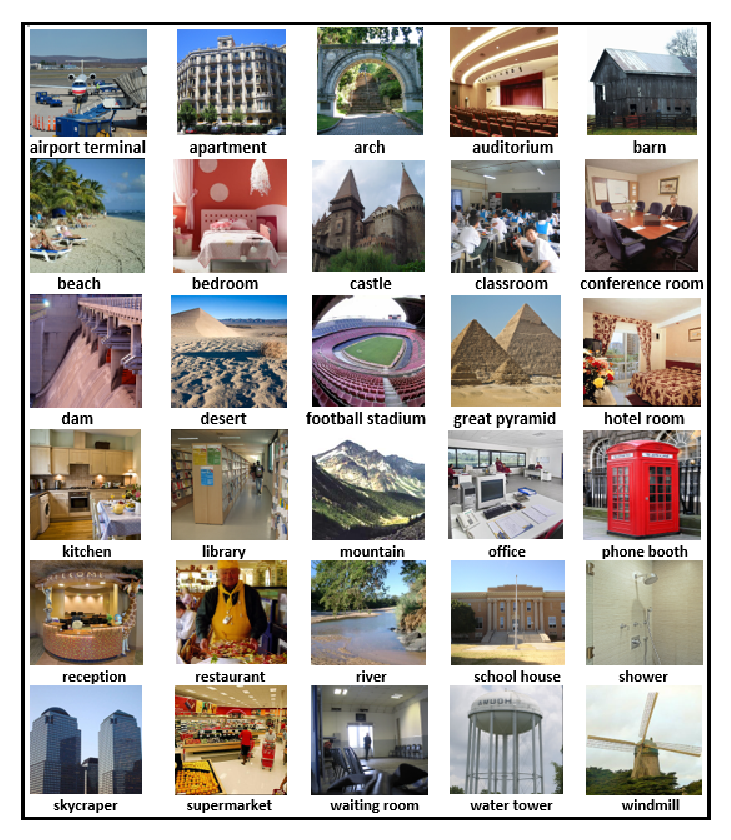
\includegraphics[width=0.7\linewidth]{SampleImages}
}
\subfigure[Example 3D scene models]
{
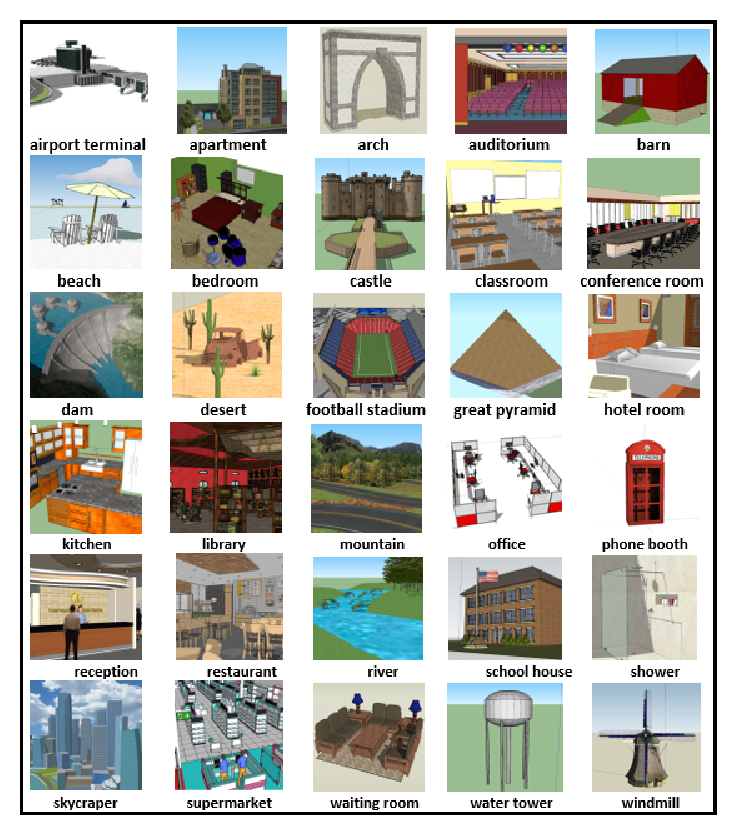
\includegraphics[width=0.7\linewidth]{SampleModels}
}
\caption{Example 2D scene sketches/images and 3D scene models in our \textbf{Scene\_SBR\_IBR} benchmark. One example per class for sketches/images/models.}
\label{BenchmarkExamples}
\end{figure}
